\section{Resultados}\label{sec:figs}

A seguir serão abordados os principais resultados obtidos através da
simulação realizada.

A Figura \ref{fig:Epidemico_SocialRoute} mostra o resultado com relação
ao tempo de entrega das mensasens considerando os protocolos Epidêmico e
o protocolo SocialRoute. Os resultados estão apresentados através de uma
CDF (Cumulative Distribution Function). O tempo de entrega é referente
ao tempo de entrega de cada mensagem enviada na simulação. Valores
negativos indicam que a mensagem não foi entregue. Podemos observar com
o auxílio dessa figura que, utilizando o protocolo Epidêmico para
entrega das mensagens, aproximadamente 70\% das mensagens foram
entregues em até 1000 rounds. Podemos observar ainda que nem todas as
mensagens foram entregues ao destinatário. Apesar disso, esse protoco
obteve um desempenho muito superior em relação ao algoritmo proposto,
SocialRoute (Descrito na seção \ref{algoritmos}). O SocialRoute não foi
capaz de entregar nenhuma mensagem ao destinatário no período
analiasado. Existem algumas explicações para esse resultado, dentre elas
o fato de que no no dataset analisado amigos não se encontraram com alta
frequência. Como o SocialRoute é baseado apenas no quesito de amizade
para a entrega das mensagens resultou em um desempenho insatisfatório.
Uma adaptação que pode ser considerada nesse protocolo é a entrega de
mensagens também para os estranhos familiares, além dos amigos. Essa
estratégia será discutida posteriormente.

\begin{figure}[ht]
\centering
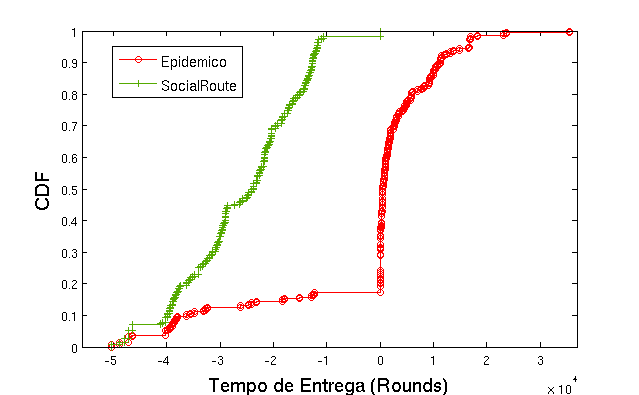
\includegraphics[width=.7\textwidth]{img/tempo_epidemico_socialRoute.png}
\caption{Tempo de entrega das mensasens considerando os protocolos Epidêmico e SocialRoute}
\label{fig:Epidemico_SocialRoute}
\end{figure}

% \begin{figure}[ht]
% \centering
% 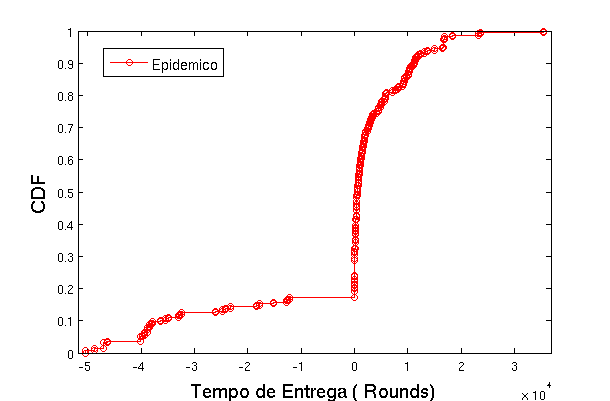
\includegraphics[width=.7\textwidth]{img/tempo_epidemico_solo.png}
% \caption{Tempo de entrega das mensasens considerando o protocolo Epidêmico}
% \label{fig:EpidemicoSolo}
% \end{figure}

A Figura~\ref{fig:Epidemico_EpidemicoNetCode} mostra os resultados
referentes ao tempo de entrega das mensasens considerando o protocolo
Epidêmico e Epidêmico utilizando codificação em rede. Podemos observar
que o desempenho da versão do algoritmo Epidêmico que utiliza
codificação em rede foi inferior quando comparado com a versão que não
utiliza esse mecanismo. Como descrito anteriormente, ao utilizar
codificação em rede na entrega das mensagens, um nodo espera um
intervalo de tempo com o intuito de codificar várias mensagens um uma
só. Com isso, um resultado inferior, em relação à versão sem codificação
em rede, já era esperado. O que não era esperado é um resultado muito
inferior, como o obtido. Acreditamos que esse resultado precisa ser
revisto.

\begin{figure}[ht]
\centering
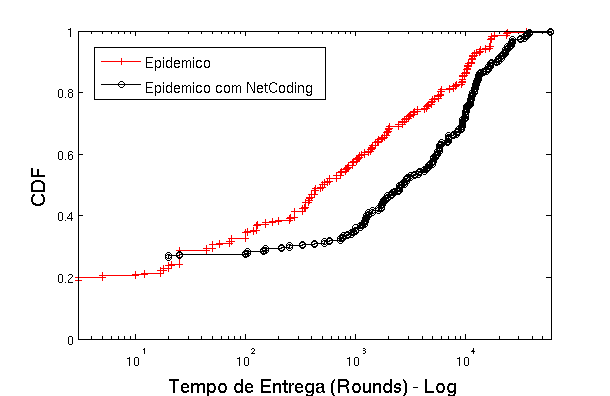
\includegraphics[width=.7\textwidth]{img/tempo_epidemico_EpidemNetCode.png}
\caption{Tempo de entrega das mensasens considerando o protocolo Epidêmico e Epidêmico com codificação em rede}
\label{fig:Epidemico_EpidemicoNetCode}
\end{figure}

Uma última análise realizada considerou um cenário com interferências na
comunicação. A Figura \ref{fig:Epidemico_EpidemicoNetCode_interf} mostra
os resultados dessa análise. Nessa figura é mostrado os resultados do
algoritmo Epidêmico sem interferências na comunicação e com
interferências na comunicação.  O eixo X dessa figura está na escala
logaritmica, mostrando apenas mensagens que foram enviadas.  É possível
observar que a entrega das mensagens é muito prejuticada sob
interferências. O Epidêmico conseguiu entregar apenas 8 mensagens ao
destinatário. Esse resultado é parcialmente influenciado pelo intervalo
de tempo considerado na simulação. De qualquer forma uma rede nessas
condições não funcionaria de maneira aceitável.

\begin{figure}[ht]
\centering
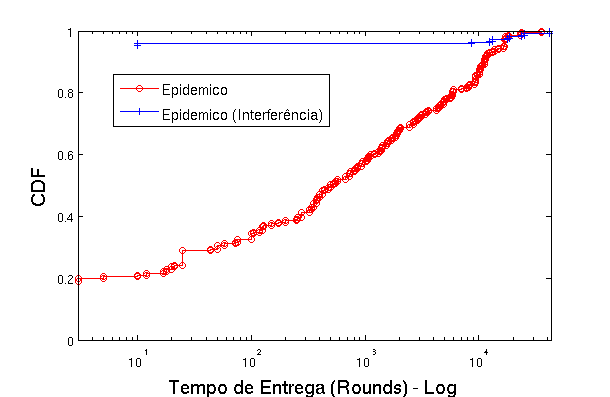
\includegraphics[width=.7\textwidth]{img/tempo_epidemico_interferencia.png}
\caption{Tempo de entrega das mensasens considerando o protocolo Epidêmico e Epidêmico com codificação em rede, em um cenário com interferência}
\label{fig:Epidemico_EpidemicoNetCode_interf}
\end{figure} 
